\documentclass[./../../paper.tex]{subfiles}
\graphicspath{{\subfix{./../../figures/}}}

\begin{document}


For the experiment, we chose a termination point of \optional{200} which is twice the length of the previous simulation. We keep the mutation rate at \optional{0.01} for each mutation type. The remaining procedure follows the process described in \autoref{sec:exp1}.

\begin{figure}[htbp]
    \centering
    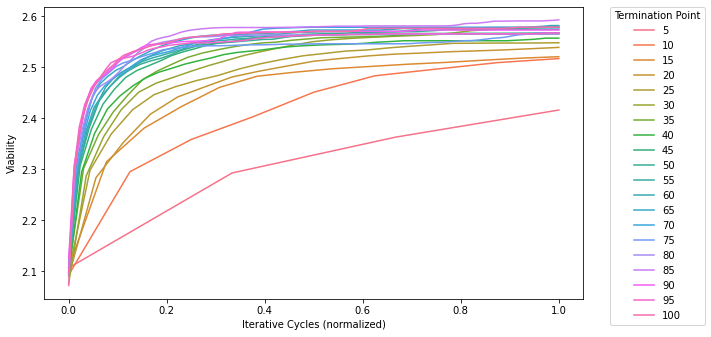
\includegraphics[width=\textwidth]{figures/generated/exp3_relative_cycles.png}
    \caption{This figure shows the viability across the iteration cycles.}
    \label{fig:exp3-normalised-lineplot}
\end{figure}

In \autoref{fig:exp3-normalised-lineplot}, we see a general increase in viability for each termination point. It shows that increasing the termination point also yields better results at the end of the generation process. 
We see that \optional{CBI-ES-UC3-SBM-RR} returns the best results in the shortest time span. The model converges after roughly 50 iterative cycles. \optional{CBI-RWS-OPC-SBM-BBR} appears to have not reached convergence. 
The randomly initiated models have not reached convergence as well. However, they remain far below models that use a more sophisticated method to initialise their population. 

\begin{figure}[htbp]
    \centering
    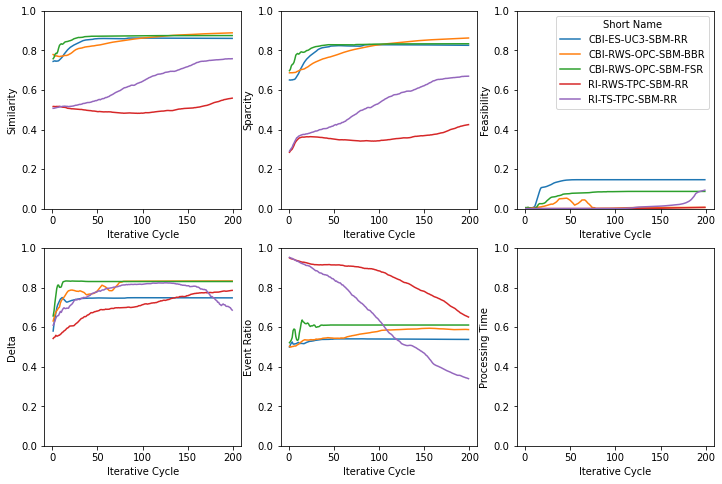
\includegraphics[width=\textwidth]{figures/generated/exp3_cycles_components.png}
    \caption{This figure shows the remaining measure components. Additionally, we show the ratio of events within the population. We also show a magnified version of the feasibility measure.}
    \label{fig:exp3-components}
\end{figure}

\autoref{fig:exp3-components} shows a decomposed view on how the viability measure evolves. Furthermore, we show the average amount of events within a generated counterfactual. 
In terms of similarity and sparsity, all models behave similarly. This is no surprise as both measures are inherently interlinked. 
We see that the randomly initiated models (RI-x) decrease the number of events they generate. 
Case-based initiated models appear to gain more viability slightly. Although,  \optional{CBI-RWS-OPC-SBN-BBR} appears that reaches its saturation point significantly later (\optional{100}th cycle).
Interestingly, the \optional{CBI-RWS-OPC-SBM-BBR} model struggles to maintain feasibility and collapses to near 0 after the \optional{100th} iterative cycle. 
Another surprise is the steep ascension of the only model that uses tournament selection (\optional{RI-TS-TPC-SBM-RR}) towards the end of the generation process. The model even overtakes the model that leads the model configurations in terms of \optional{viability}. 
Furthermore, we see that \optional{CBI-ES-UC-SBM-RR} has the highest feasibility among all models. However, it also quickly converges after 50 iterative cycles.    
   

% \begin{figure}[htbp]
%     \centering
%     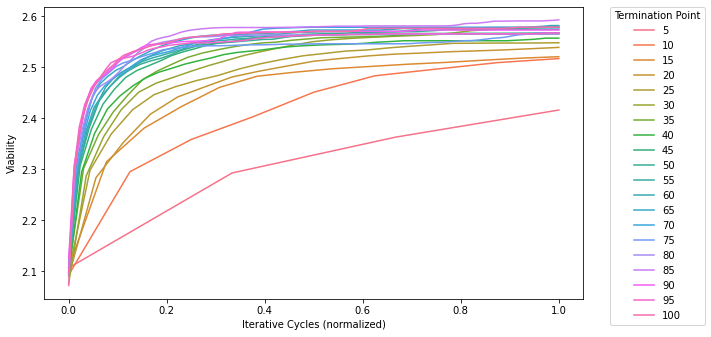
\includegraphics[width=\textwidth]{figures/generated/exp3_relative_cycles.png}
%     \caption{shows the viability reached given the termination point. All termination points are normalised for better comparability.}
%     \label{fig:exp3-iterations-boxplots}
% \end{figure}


% Furthermore, in \autoref{fig:exp3-iterations-boxplots} reflects the spread of the individual results. Unsurprisingly, low termination points yield a larger spread dispersion of viability. The values become less dispersed, and the higher the termination point. \optional{However, there are some surprising outliers. First, the termination points 55, 60 and 90 seem to have an extremely low dispersion. Meaning most of their results have the same viability. It is not clear whether this is a rule or a mere coincidence.} Also, the number of outliers increases with the termination point as well. The last noteworthy observation is the number of solutions near the mark of \attention{1.8}, as depicted with the dotted line.

\end{document}